\documentclass[10pt, a4paper]{article}
\usepackage{lrec2006}
\usepackage{graphicx}
\usepackage{todonotes}
\newcommand{\ryan}[1]{\todo[color=green!40,author=Ryan]{#1}}
\title{A Multi-Dialect, Multi-Genre Corpus of Informal Written Arabic}

\name{Ryan Cotterell,$^1$ Chris Callison-Burch$^2$}
\address{ 
 $^1$ Center for Language and Speech Processing, Johns Hopkins University \\
 $^2$ Computer and Information Science Department, University of Pennsylvania}
%              \{ryan.cotterell, adithya.renduchintala,nsaphra\}@jhu.edu; ccb@cis.upenn.edu}


\abstract{
This paper presents a multi-dialect, multi-genre, human annotated
corpus of dialectal Arabic with data obtained from both online newspaper
commentary and Twitter. Most Arabic corpora are small and focus on
Modern Standard Arabic (MSA). There has been recent interest, however,
in the construction of dialectal Arabic corpora
\cite{zaidan2011arabic,al2012yadac}. This work differs from previously 
constructed corpora in
two ways. First, we include coverage of five dialects of Arabic:
Egyptian, Gulf, Levantine, Maghrebi and Iraqi. This is the most
complete coverage of any dialectal corpus known to the authors.  In
addition to data, we provide results for the Arabic dialect
identification task that outperform those reported in \newcite{zaidan2011arabic}.
\\ \newline
\Keywords{arabic, dialectal arabic, dialect identification, crowd-sourcing annotation}}



\begin{document}

\maketitleabstract

\section{Introduction}
This paper presents a multi-dialect, multi-genre, human annotated
corpus of dialectal Arabic with data obtained from both online newspaper
commentary and Twitter. Most Arabic corpora are small and focus on
Modern Standard Arabic (MSA). There has been recent interest, however,
in the construction of dialectal Arabic corpora
\cite{zaidan2011arabic,al2012yadac} . This work differs from these in
two ways. First, we include coverage of five dialects of Arabic:
Egyptian, Gulf, Levantine, Maghrebi and Iraqi. This is the most
complete coverage of any dialectal corpus known to the
authors. Second, every sentence in the corpus was human annotated on
Amazon's Mechanical Turk; this stands in contrast to
\newcite{al2012yadac} where only a small subset was human annotated in
order to train a classifier. In addition to data, we provide results for
the Arabic dialect identification task that outperform those reported in
\newcite{zaidan2011arabic}. The paper is structured as follows:
in section \ref{sec:arabic} we provide a brief overview of the
relevant socio-linguistic details of the Arabic language, in section
\ref{sec:related} we discuss related work pertaining to dialect corpus
creation and dialect identification, in sections
\ref{sec:newspaper}, \ref{sec:twitter} and \ref{sec:annotation} we discuss our 
methodology and
annotation techniques and in section \ref{sec:experiments} 
we discuss experiments.


\section{Arabic}\label{sec:arabic}
Arabic exhibits a linguistic phenomenon known as diglossia, in which
the written standard differs substantially from the spoken
vernacular. The written standard, known as Modern Standard Arabic
(MSA), is largely based on the Qur'anic literary register. It is used
across the Arabic-speaking world in written news and in broadcast media. The
local dialects however, differ substantially from MSA at all
linguistic levels. The recent emergence of informal, user-generated
text has led to a proliferation of large quantities of written
dialectal Arabic on the internet. The Arabic dialects differ for
historical reasons and have been individually influenced by the
pre-Arabization language spoken by the population, as is the case with
Aramaic in the Levant, as well as the European languages from the time
of colonization. Such distinctions are important as North African
dialects are unique in the quantity of French loanwords, whereas Iraqi
Arabic has been historically more influenced by Turkish.

The stark difference between MSA and the dialects creates a problem
for NLP software trained largely on MSA text. As most previous efforts
in Arabic NLP have focused on MSA, there is a dearth of resources
available to adequately tackle the problem. A natural starting place
for Arabic-dialect NLP lies in dialect identification and
classification. Since each dialect group should be treated as a
separate language from the point of view of downstream processing tasks,
classifying them will be key for any pipeline.
\begin{figure}
\centering
  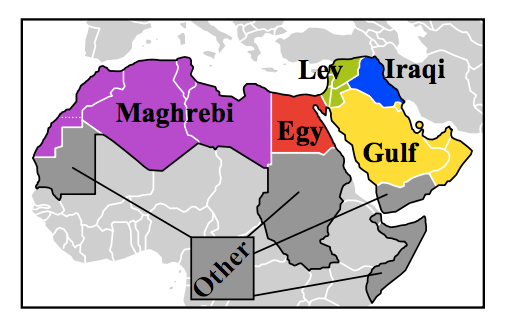
\includegraphics[width=75mm]{figs/dialect_map2.png}	
\caption{Arabic Map}
\end{figure} 
At the highest level, the Arabic dialects can be divided into two
groups: the \textit{maghreb} and the \textit{mashreq} dialects. The
\textit{maghreb} dialects consist of the North African dialects spoken west of
Egypt and the \textit{mashreq} dialects include everything east of
Egypt. Within these broader categories, subdivisions are made whose
differences often reflect pre-Arab culture and colonial history. We
opted to classify dialect Arabic into five groups
	\begin{description}
		\item \textbf{Maghrebi} (spoken in all of North
Africa)
		\item \textbf{Egyptian} (spoken in Egypt, but
understood universally)
		\item \textbf{Levantine} (spoken primarily in the
Levant, Syria and Palestine)
		\item \textbf{Iraqi} (spoken in Iraq)
		\item \textbf{Gulf} (spoken primarily in Saudi Araubi,
UAE, Kuwait and Qatar)
	\end{description}
	
Automatically, identifying dialects is a more complex task than
language identification. The relation between Latin and Romance
languages is often brought forth as a European equivalent of the
distinction between the MSA and the Arabic dialects. However, Arabic
dialect identification is further complicated by the
orthography. Traditionally, vowels are omitted from Arabic text
leaving obvious phonological clues absent. A similar task would be
stripping the vowels from French and Italian text and trying to
identify the correct language. A further complication arises in the
shared technical vocabulary from MSA.


\section{Related Work}\label{sec:related}
Our work is a direct extension of \cite{zaidan2011arabic} in that we
use a similar methodology for the collection of the data and the
classification task. There are several other dialectal Arabic corpora
of note. \newcite{al2012yadac} created an Egyptian Arabic corpus through
human annotation and classifiers.  The COLABA project has similarly
constructed dialectal resources from web logs
\cite{diab2010colaba}. \newcite{elfardy2012simplified} provide
guidelines for the construction of large corpora of mixed Arabic
resources. \newcite{elfardy2012AIDA} introduced AIDA, a system for
dialect identification, classification and glossing on both the token
and sentence level. \newcite{elfardy2013sentence} presented a
supervised approach for sentence level dialect identification and
studied the effects of preprocessing techniques on classifier
accuracy. \newcite{tratz2013tweet} made efforts to improve the
annotation of Arabic corpora through the creation of a tool specifically
designed to facilitate the annotation of social media data. A different
line of work that is relevant is the analysis of code-switched
data. Owning to the informal nature of conversations in Arabic
dialects, the language is often mixed with MSA. Therefore the line
between what is dialect and what is MSA is
blurred. It thus may be more appropriate to consider the task of token level
dialect identification as in \newcite{elfardy2012token}.

\section{Newspapers}\label{sec:newspaper}
We set out to create a dataset of dialectal Arabic to address the general
lack of resources. The most viable resource of dialectal Arabic text is online
data, which is more individual-driven and less institutionalized, and
therefore more likely to contain dialectal content. Possible sources
of dialectal text include web logs, fora, and chat transcripts.
 We collected
a substantial amount of dialect data from user comments from online
newspapers, following \newcite{zaidan2011arabic} We chose 5 Arabic
language newspapers for this commentary set: an Egyptian newspaper
\textbf{Al-Youm Al-Sabe'}, a Saudi-Arabian newspaper
\textbf{Al-Riyadh}, a Jordanian newspaper \textbf{Al-Ghad}, an
Algerian newspaper \textbf{Ech Chorouk El Youmi} and an Iraqi
newspaper \textbf{Al-Wefaq}.


\section{Collection of Twitter Data}\label{sec:twitter}

% You really need to describe the Twitter API?  The popularity of
Twitter (\texttt{twitter.com}) has provided researchers with an
enormous quantity of natural language data. In particular, Twitter is
an excellent source for colloquial data in many languages. Users
typically tweet short, informal messages that reveal many properties
of spoken languages \cite{eisenstein2013phonological}. Twitter data
varies substantially from newspaper commentary, making it a natural complement
to the previously scraped data since the service imposes a 140 character limit
on all messages, which encourages non-standard orthography.
\\
Twitter provides a well-documented streaming API that allows easy access to their
social media content. %There are different APIs, such as the REST API
%and the streaming API. %The REST API is generally not of use for
%scraping large volumes of tweets as it is designed for interactive
%websites.
 % The streaming API is more appropriate since it offers low
% latency access to Twitter's \textit{global stream} of Tweet
% data. There are three types of streams: public streams, user streams
% and site streams. Public streams contain \textit{all} public following
% through Twitter and user streams are a multi-user version of user
% streams. %This sentence is probably wrong. Unless you actually mean
% that user streams are multi-user version of user streams Public
% streams are most useful if the goal is to glean a large random sampler
% of Twitter streams subject to certain constraints. % I altered this
% sentence, but you should probably make sure this sentence means what
% you want to mean
Access to the Twitter API is rate limited, however, and no individual stream may
contain more than 1\% of the total global stream. 
%Given the uneven
%distribution of tweets from different parts of the world, this is
%generally not a problem. 
Since the number of Arabic-language
tweets as a percentage of the global stream is much less than 1\%,
this generally is not a problem.

%\begin{figure}
%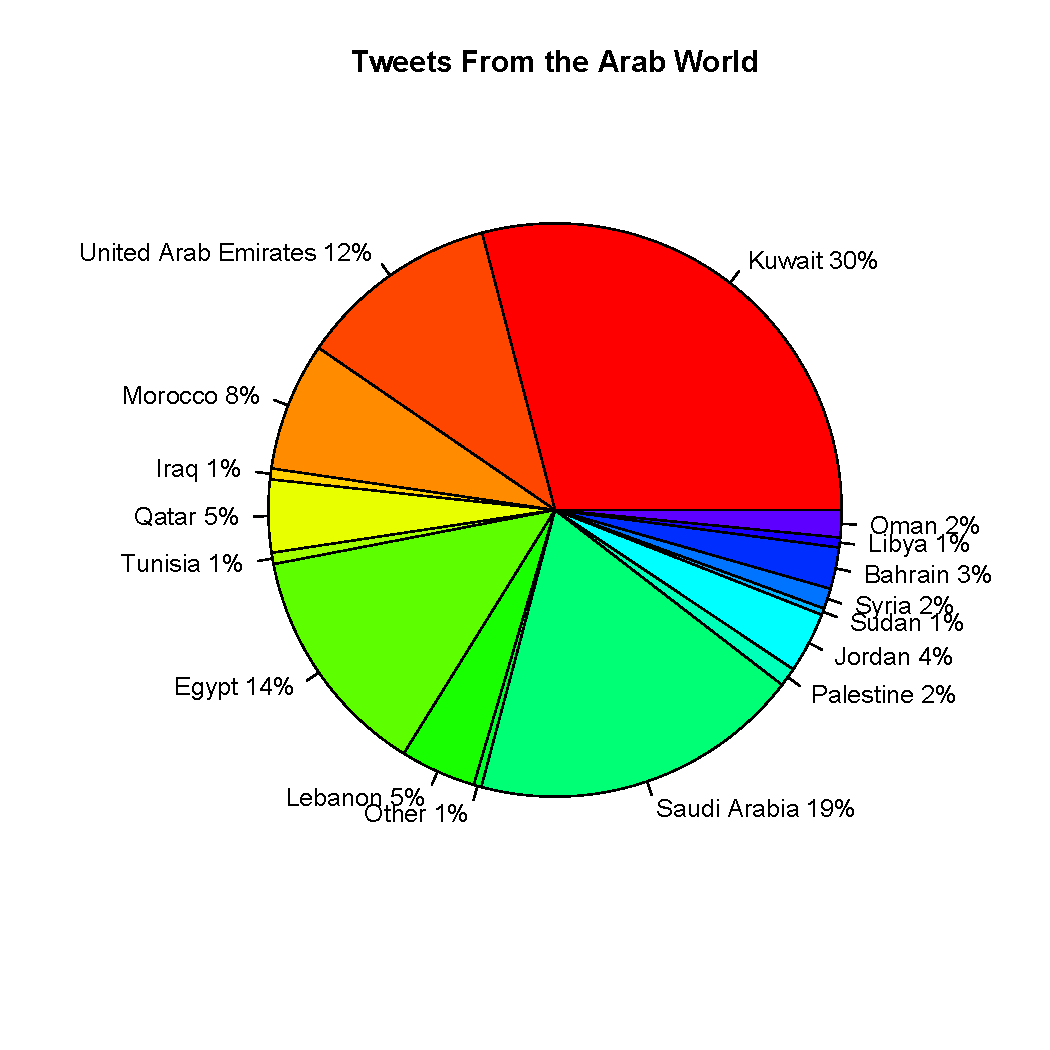
\includegraphics[scale=0.5]{figs/tweets_from_the_arab_world.pdf}
%\caption{Distribution Of Arabic Tweets By Country}
%\end{figure}
\section{Annotation}\label{sec:annotation}
Amazon's Mechanical Turk (MTurk) provides the primary annotation
platform. MTurk has recently been exploited for large-scale linguistic
annotation \cite{callison2010creating,zaidan2011crowdsourcing}. MTurk
provides an environment in which ``requesters'' can set up Human
Intelligent Tasks (HITs) to be performed by ``workers''. The tasks
typically require human knowledge. To interact with the workers, the
requester creates an interactive website that allows the
``worker'' to perform the task. We randomly divided the sentences into
groups of 10 and additionally provided 2 controls, which trusted
annotators had previously labeled. The controls were selected from the
Arabic Online Commentary Dataset \cite{zaidan2011arabic}.  The controls
were only marked for dialect versus MSA, a much easier task than
dialect identification.  Each HIT required a worker to give a judgment
to specify which dialect (including MSA) the message was written in as
well as the ``dialectness'' of the tweet.  We gave each worker 60
minutes to complete the task from start to finish although the average
time was substantially less than this. Additionally, we required the
workers to fill out a brief survey about their native language, place
of birth and current place of residence.
\\
To ensure the quality of the annotation, we monitored performance on
the controls. For full payment, we required that the worker achieve
85\% accuracy on the control. Most workers, however, achieved well
above that mark. Workers who performed better than chance, but below
the 85\% threshold were compensated proportionally for the number of
correct annotations
\\
Two main groups of HITs were put up: one for the newspaper commentary
and one for the twitter data. The design was the same and is pictured
in Figure 2. Both of these hits required approval to access, which
was granted on the basis of performance on an
identical ``test'' HIT with the exception that no restriction was
applied. Workers who performed well on the ``test'' were then granted
the qualification on the main HIT. Each group consisted of 100,000
messages from the commentary data set and from Twitter respectively.
\\
230 workers attempted the ``test'' HIT. Of those 230, 23 passed the
initial qualification. All of these workers self-reported speaking
Arabic natively, although not all resided in Arabic speaking countries. 
The 23 workers completed all the HITs in both groups over a 4
month period. Figures \ref{fig:performance1} and \ref{fig:performance2} 
show the performance of the individual workers on newspaper commentary
annotation task and the tweet annotation task.


% Is it ok to have informal language like this? 

\begin{figure*}
\centering
\setlength\fboxsep{0pt}
\setlength\fboxrule{0.25pt}
  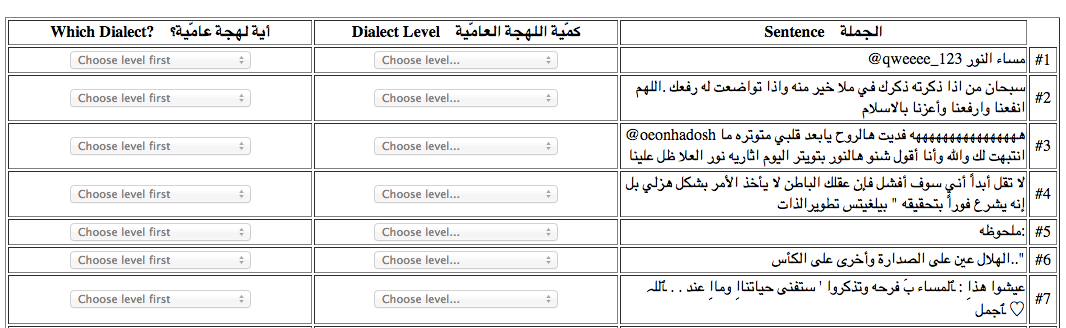
\includegraphics[width=1.00\linewidth ]{figs/hit_screenshot}	
\caption{Screenshot of HIT}
\label{f7}
\end{figure*}


%\begin{figure}
%  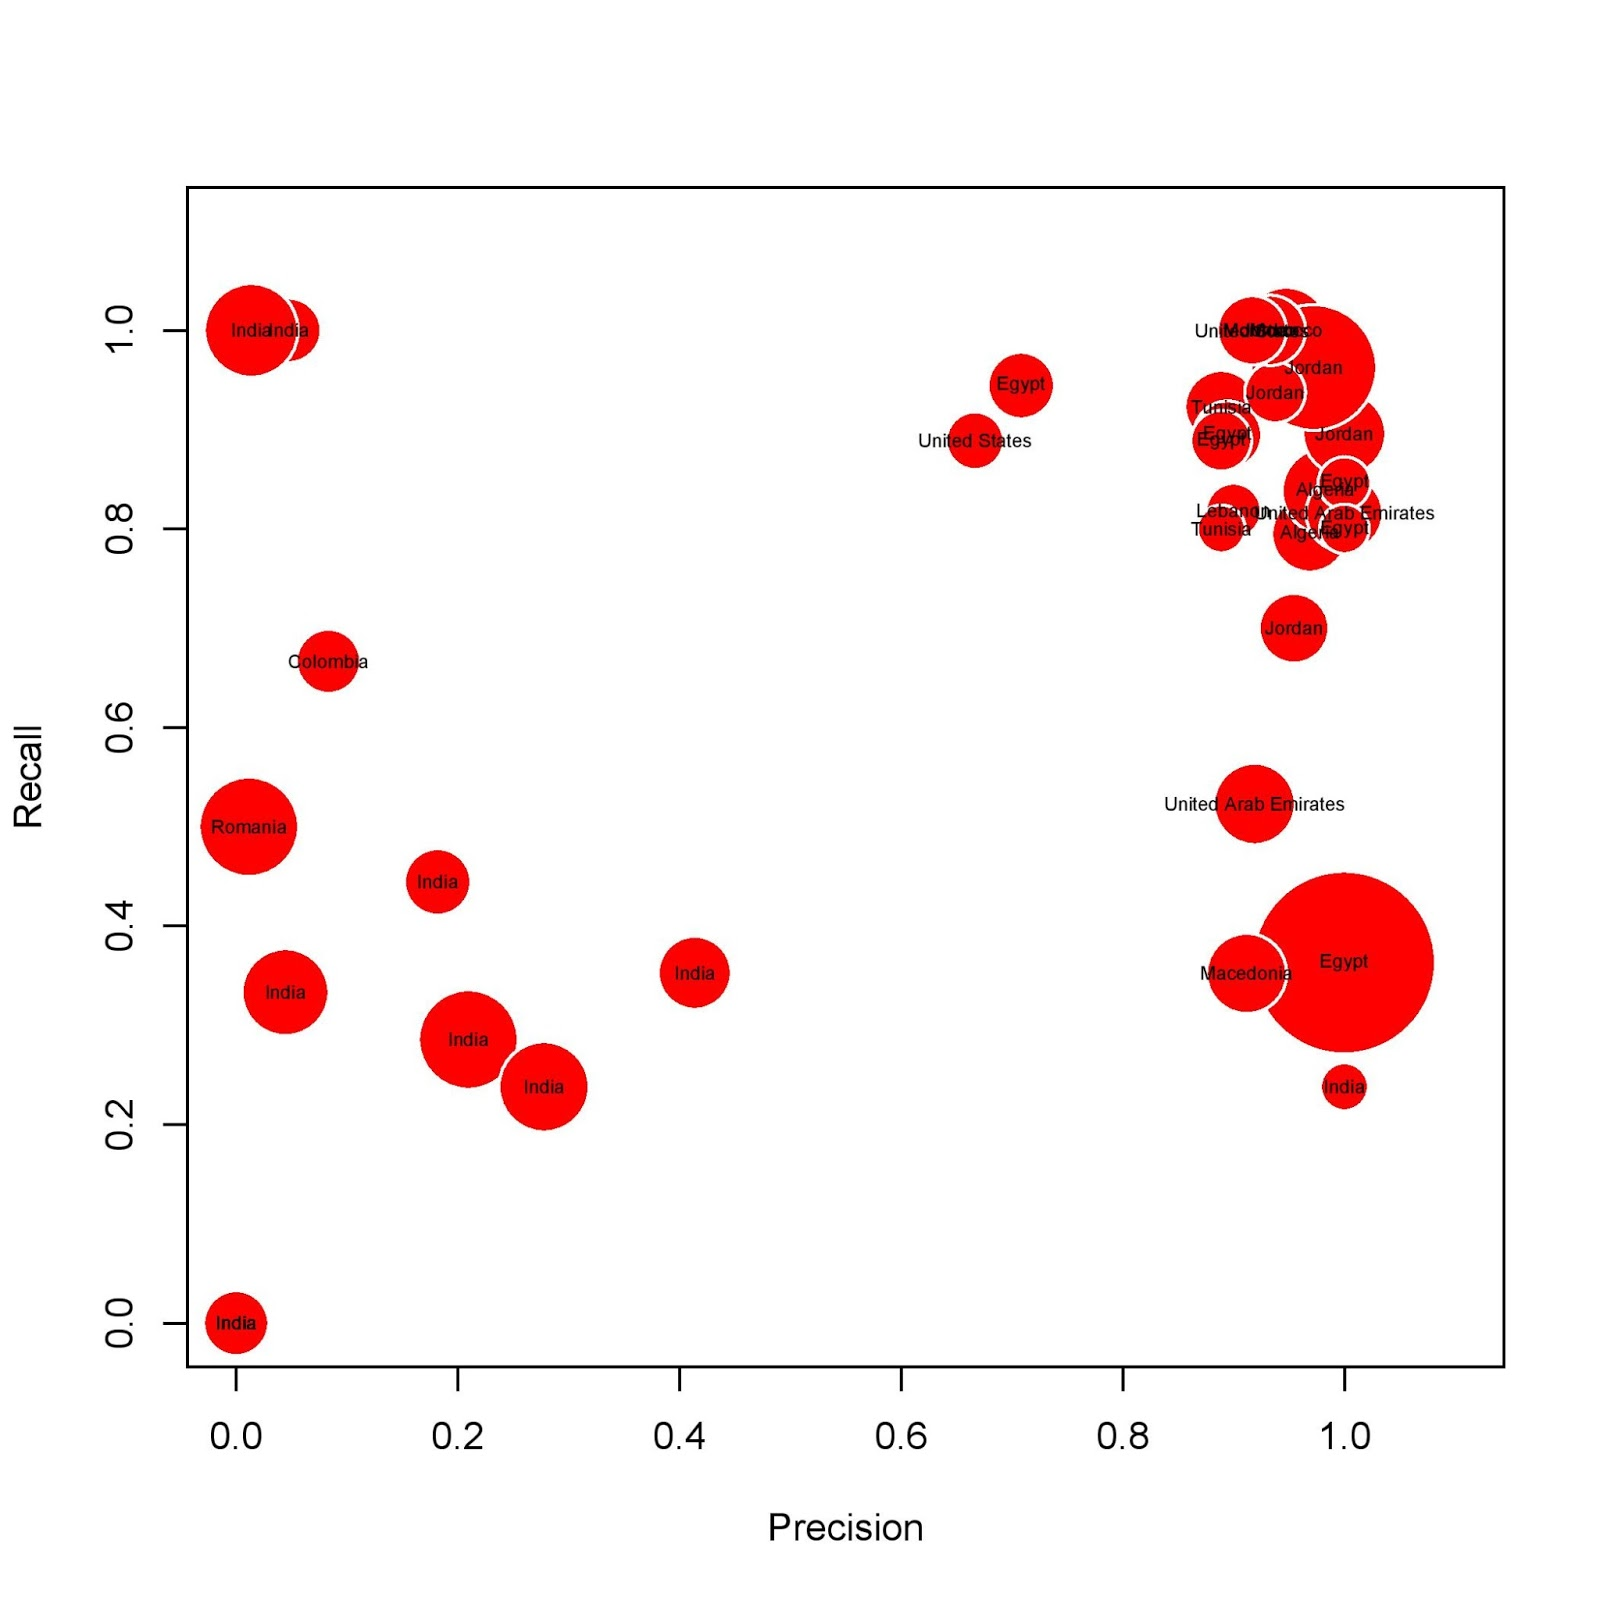
\includegraphics[width=75mm]{figs/all_turkers-page-001.jpg}	
%\caption{Precision/Recall labeled by Country}
%\end{figure} 

\begin{figure}
\centering
\begin{tabular}{|c|c|c|c|c|c|} \hline 
& Comments & Words \\ \hline 
\textit{Al-Ghad} & 4811 & 100K \\ \hline
\textit{Al-Riyadh} & 6307 & 105K \\ \hline
\textit{El-Youm El-Sabe3} & 8927 & 220K \\ \hline
\textit{Al-Wifaq} & 254 & 8K \\ \hline
\textit{Echourouk} & 6940 & 150K \\ \hline
\end{tabular}
\caption{Newspaper commentary annotated on MTurk as having high dialectal content}
\end{figure}


\begin{figure}
\centering
\begin{tabular}{|c|c|c|c|c|c|} \hline 
& Tweets & Words \\ \hline 
\textit{Levantine} & 1594 & 22K \\ \hline
\textit{Gulf} & 36330 & 611K \\ \hline
\textit{Egyptian} & 2052 & 27K \\ \hline
\textit{Iraqi} & 154 & 4K \\ \hline
\textit{Maghrebi} & 99 & 2K \\ \hline
\end{tabular}
\caption{Tweets annotated on MTurk as having high dialectal content}
\end{figure}



\begin{figure}
\centering
\begin{tabular}{|c|c|c|c|c|c|} \hline 
Country & \# Hits  & Acc. 	& Prec. & Rec. & F1\\ \hline
Algeria & 198 & 0.96 & 0.97 & 0.98 & 0.98 \\ \hline
Algeria & 2 & 1.0 & 1.0 & 1.0 & 1.0 \\ \hline
Algeria & 4 & 1.0 & 1.0 & 1.0 & 1.0 \\ \hline
Egypt & 11 & 0.91 & 0.89 & 1.0 & 0.94 \\ \hline
Egypt & 1264 & 0.95 & 0.96 & 0.98 & 0.97 \\ \hline
Egypt & 743 & 0.91 & 0.9 & 0.99 & 0.94 \\ \hline
Georgia & 43 & 0.93 & 0.92 & 1.0 & 0.96 \\ \hline
Greece & 193 & 0.95 & 0.98 & 0.95 & 0.97 \\ \hline
Jordan & 1228 & 0.97 & 0.96 & 0.99 & 0.98 \\ \hline
Jordan & 3160 & 0.96 & 0.96 & 0.99 & 0.97 \\ \hline
Lebanon & 62 & 0.95 & 0.98 & 0.96 & 0.97 \\ \hline
Morocco & 673 & 0.95 & 0.95 & 0.99 & 0.97 \\ \hline
Morocco & 732 & 0.95 & 0.99 & 0.95 & 0.97 \\ \hline
Tunisia & 2104 & 0.92 & 0.97 & 0.93 & 0.95 \\ \hline
Tunisia & 28 & 0.82 & 0.98 & 0.82 & 0.89 \\ \hline
Tunisia & 3766 & 0.96 & 0.97 & 0.97 & 0.97 \\ \hline
U.K. & 1193 & 0.96 & 0.97 & 0.98 & 0.97 \\ \hline
U.S. & 1668 & 0.95 & 0.94 & 0.99 & 0.96 \\ \hline
U.S. & 20 & 0.97 & 0.97 & 1.0 & 0.99 \\ \hline
U.S. & 2407 & 0.97 & 0.96 & 0.99 & 0.98 \\ \hline
U.S. & 5 & 0.9 & 1.0 & 0.88 & 0.93 \\ \hline
\end{tabular}
\caption{Workers' Performance on Twitter HIT}
\label{fig:performance1}
\end{figure}


\begin{figure}
\centering
\begin{tabular}{|c|c|c|c|c|c|} \hline 
Country & \# Hits  & Acc. 	& Prec. & Rec. & F1\\ \hline
Algeria & 1048 & .96 & .96 & .93 & .94 \\ \hline
Egypt & 137 & .94 & .86 & .97 & .91 \\ \hline
Egypt & 139 & .9 & .74 & 1.0 & .85 \\ \hline
Egypt & 141 & .96 & .95 & .94 & .95 \\ \hline
Egypt & 4 & .75 & .5 & 1.0 & .67 \\ \hline
Egypt & 461 & .96 & .95 & 0.92 & .94 \\ \hline
Egypt & 722 & .94 & .92 & .92 & .92 \\ \hline
Greece & 416 & .9 & .97 & .79 & .87 \\ \hline
Jordan & 272 & .82 & .78 & .7 & 0.74 \\ \hline
Jordan & 417 & .97 & .96 & .95 & .96 \\ \hline
Jordan & 50 & .91 & .97 & .8 & .88 \\ \hline
Jordan & 93 & .96 & .94 & .96 & .95 \\ \hline
Lebanon & 136 & .96 & .96 & .92 & .94 \\ \hline
Morocco & 473 & .97 & .94 & .95 & .94 \\ \hline
Tunisia & 1404 & .9 & .96 & .8 & .87 \\ \hline
Tunisia & 260 & .91 & .91 & .84 & .88 \\ \hline
Tunisia & 727 & .84 & .89 & .74 & .81 \\ \hline
U.K. & 3 & 1.0 & 1.0 & 1.0 & 1.0 \\ \hline
U.K. & 828 & .95 & .93 & .91 & .92 \\ \hline
U.S. & 1337 & .95 & .89 & .98 & .93 \\ \hline
U.S. & 30 & .95 & .96 & .92 & .94 \\ \hline
U.S. & 899 & .97 & .97 & .94 & .95 \\ \hline
\end{tabular}
\caption{Workers' Performance on Arabic Commentary HIT}
\label{fig:performance2}
\end{figure}


% \section{Data}
% The data are provided in two formats. Firstly, they are provided in an
% XML format that is consistent with format from
% \newcite{zaidan2011arabic} . Additionally, we have provide the data in
% JSON format. In addition to the messages themselves, both Twitter and
% news commentary, meta-data from the poster and context is also
% provided.  The data is freely avalaible to the public \footnote{put
% the url here}.

\section{Automatic Dialect Classification}\label{classification} In
addition to the corpus, this work also budges the state of the art in
dialect identification.  Arabic dialect identification is effectively
the task of language identification, with the added difficulty that
dialects are far more similar.  In contrast to \cite{zaidan2011arabic}
, which made use of a language model for the task, we consider Naive
Bayes and Support Vector Machines. We
further extend the task to include 5 dialects in total, as opposed to
three.



\begin{figure}
\centering
  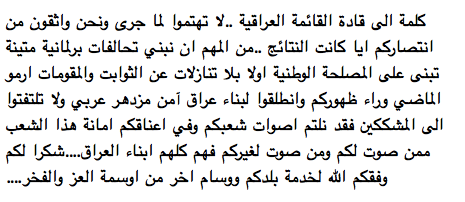
\includegraphics[width=75mm]{figs/arabictext2.png}	
\caption{Sample Commentary}
\end{figure} 


%\section{Code-Switched Arabic}
%NEED TO FORMAT

%s'il te plais chorouk ma tzidouch tenchrounna ta3ali9 ta3 lemrarka lemcharkin, a lemrarka occupez vous de vos fesses , et rohou ta3bdou el malik mouhamùadine essadisse ra3ahou llahou wa 7afidahou wa adkhalahou lahou fas7a eljinani ...etc rahou ilah ta3kom


\section{Experiments}\label{sec:experiments}
We made use of the Python-based Machine Learning library Scikit-learn
to train a classifier for the Arabic social media data
\cite{pedregosa2011scikit}. Scikit-learn provides a suite of
supervised learning algorithms that can be readily substituted in a
generic framework. We used unigram, bigram, and trigram features for
the model in combination with the two learning algorithms: SVM with a
linear kernel and Naive Bayes. We were primarily interested in the
binary classification problem dialect versus MSA with all 
five dialects. We performed 10-fold
cross-validation with each algorithm.  Accuracy is reported in figures
\ref{exp:newspaper} and \ref{exp:twitter}.

\begin{figure} \centering
\begin{tabular}{|c|c|c|c|c|c|} \hline & Egy. & Lev. & Mag. & Gulf &
Iraqi \\ \hline NB Uni & \textbf{.89} & \textbf{.79} & \textbf{.92} &
\textbf{.88} & \textbf{.87} \\ \hline NB Bi & .88 & .78 & .89 & .84 &
.66 \\ \hline NB Tri & .88 & .77 & .88 & .84 & .65 \\ \hline SVM Uni &
.88 & .78 & .89 & .85 & 85 \\ \hline SVM Bi & .87 & .75 & .87 & .82 &
.79\\ \hline SVM Tri & .87 & .74 & .87 & .82 & .79 \\ \hline
\end{tabular}
\label{exp:newspaper}
\caption{Experiments on Extended AOC (accuracy reported)}
\end{figure}

\begin{figure} \centering
\begin{tabular}{|c|c|c|c|c|c|} \hline & Egy. & Lev. & Mag. & Gulf &
Iraqi \\ \hline NB Uni & \textbf{.84} & \textbf{.84} & .70 &
\textbf{.87} & \textbf{.79} \\ \hline NB Bi & \textbf{.84} &
\textbf{.84} & \textbf{.71} & .86 .& \textbf{.79} \\ \hline NB Tri &
.83 & .74 & .70 & .86 & .65 \\ \hline SVM Uni & .80 & .81 & .65 & .86
& 75 \\ \hline SVM Bi & .79 & .76 & .57 & .86 & .62\\ \hline SVM Tri &
.77 & .76 & .57 & .86 & .62 \\ \hline
\end{tabular}
\label{exp:twitter}
\caption{Experiments on Twitter (accuracy reported)}
\end{figure}

We observe that the unigram models typically outperform the higher
order models; the additional features hurt the model performance. This is 
 surprising; it
is possible that dialectal words do not typically occur in sequence
and it is therefore bigrams and trigrams do not help
performance. Another explanation could stem from the informal nature
of the text. The varying orthorgrahical conventions typically increase
sparsity and make it more difficult to estimate the true $n$-gram
probabilities. We also compared our model to
\newcite{zaidan2011arabic}. We trained our best performing model,
Naive Bayes with unigram features, on the data released with
\newcite{zaidan2011arabic} and showed significant improvements.
The numbers are reported in table \ref{tab:comparison}.
\begin{figure} \centering
\begin{tabular}{|c|c|c|} \hline & NB & Zaidan et al. (2011a) \\
\hline MSA vs. Lev. & 86.6 & 79.6 \\ \hline MSA vs. Gulf & 82.7 & 75.1
\\ \hline MSA vs. Egy. & 86.6 & 80.9 \\ \hline
\end{tabular}
\label{tab:comparison}
\caption{Experiments on Extended AOC}
\end{figure}


\section{Future Work} The problem of Arabic dialect identification is
still very much an open problem despite the introduction of an
additional annotated corpus in this work. While language identification is often
considered a solved problem, \newcite{mcnamee2005language} points out
that problem can be made arbitrarily difficult by using informal text,
many languages, short text, and unbalanced data. The Arabic dialect
identification
task inherently embodies many of these attributes. Dialectal Arabic
occurs exclusively in informal text, which is often short due to the
nature of social media. Additionally, the task of Arabic dialect
identification with short messages may often be impossible. Just as an
informal message containing only the text \textit{por que?} could
either be Spanish or Portuguese, many short Arabic texts are
inherently ambiguous. Future work should attempt to define an
empirical error in human classification of data, as it is unlikely
rates similar to those seen in traditional language identification can be achieved. 
Additional efforts should also focus on isolating dialectal features from topical
features. As the source of each dialect was a single newspaper, it is
reasonable to expect that differences in $n$-gram counts are due only to
the topical coverage of each newspaper and not to inherent
differences in the dialects. It is important to mitigate the boost in accuracy attributable
to these features to get a better sense of the models' performance on
new data. One possible solution to this problem is to scrape comments
from multiple websites in the same country and compare the
corresponding accuracy. Also leveraging the vast of amount of
unannotated data is of interest. It is financially unfeasible to
annotate all the data scraped from online fora, but it nevertheless
may be possible to improve performance through the use of
semi-supervised techniques. It is also necessary to extend the
coverage of corpus to additional dialects. No data was collected from
newspapers from Sudan, which has its own distinct dialect of Arabic
\cite{comrie2013major}. Additionally, there are stark contrasts
between various North African dialects, such as between Tunisian and
Moroccan \cite{comrie2013major}.

\section*{Acknowledgements}
This material is based on research sponsored by a DARPA Computer Science Study Panel phase 3 award entitled ``Crowdsourcing Translation'' (contract D12PC00368). The views and conclusions contained in this publication are those of the authors and should not be interpreted as representing official policies or endorsements by DARPA or the U.S. Government. This research was supported by the Johns Hopkins University Human Language Technology Center of Excellence. Adithya Renduchintala acknowledges support of NSF (IIS-1349902).


\nocite{*}
\bibliographystyle{lrec2006}
\bibliography{dialect_annotation}

\end{document}

